% !TeX spellcheck = en_US
\addscenariosection{1}{Clash Scenario}{King of the Hill v2}{\images/kingofthehill.png}

\begin{multicols*}{2}

\textbf{Author:} KABLAMIO \& Cantila

\textbf{Source:} \href{https://discord.com/channels/1275490124301467799/1284428969369665631}{KABLAMIO's Discord}

\textit{Win (and lose) PvP fights and hold the Hill.}

\subsection*{\MakeUppercase{Scenario Length}}
This Scenario plays out over 6 Rounds.

\subsection*{\MakeUppercase{Player Setup}}
\textbf{Player Count:} 2 -- 3

\textbf{Starting Resources:} 22 \svg{gold}, 5 \svg{building_materials}

\textbf{Starting Income:} 15 \svg{gold}, 2 \svg{building_materials}, 1 \svg{valuables}

\textbf{Starting Units:}
\begin{itemize}
  \item Few of \silver\ with the lowest Recruitment cost.
\end{itemize}

\textbf{Town Buildings:}
\begin{itemize}
  \item \bronze\ Dwelling
\end{itemize}

\subsection*{\MakeUppercase{Map Setup}}
Take the following Map Tiles and arrange them as shown in the Scenario map layout ($P$ stands for the number of players):

\begin{itemize}
  \item P × Starting (I) Map Tile
  \item P × Far (II-III) Map Tiles
  \item P × Near (IV-V) Map Tiles
  \item Center Map Tile (C1 or C3)
  \item Custom Center Map Tile
\end{itemize}

\subsection*{\MakeUppercase{Victory Conditions}}
The game ends at the end of the Round 6.

\subsection*{\MakeUppercase{Victory Points}}
The Player with the most Victory Points (VP) wins. Players get
VPs for:
\begin{itemize}
  \item Round number - 1 VP for starting your turn on ``The Hill''
  \item 2 VP for winning a Combat against another Player
  \item 1 VP for losing a Combat against another Player
\end{itemize}

\subsection*{\MakeUppercase{Timed Events}}

\begin{itemize}
  \item \textbf{\nth{2} Round:} Gain secondary Hero for free.
  \item \textbf{\nth{3} Round:} Gain Citadel for free. If you had it, gain 1 VP.
  \item \textbf{\nth{4} Round:} Gain \silver\ dwelling for free. If you had it: gain 2 VP.
  \item \textbf{\nth{5} Round:} Gain \golden\ dwelling for free. If you had it: gain 3 VP.
\end{itemize}

\subsection*{\MakeUppercase{Additional Rules}}
\begin{itemize}
  \item Every Round after Round 1 is a Resource Round.
  \item Players can't attack their opponent's starting Town.
  \item Players can only attack another player once each turn.
  \item Players do not lose gold for losing or retreating from any Combat.
  \item Secondary Heroes act as Main Hero.
  \item After losing a Combat, the defeated Hero is moved to it's starting Town.
  \item After PvP Combat, both Players gain their lost \bronze\ and \silver\ Units back.
  \item Players may \svg{pay_v2} 6 \svg{gold} and 6 \svg{building_materials} to gain Walls and Arrow Tower until their next turn.
  \item Level VI and VII Combats cannot be skipped.
  \item Level VII Neutral Combat reward: Gain 20 \svg{gold}.
  \item \textbf{Obelisks:} Search (2) \svg{artifact}. \textit{Visitabe once per Faction.}
  \item \textbf{Dragon Utopias:} On Center Map Tile a Hero can spend 1 \svgeven{movement} to teleport to Dragon Utopia. After Flagging Dragon Utopia, gain 10\svg{gold}, resolve all rewards from adjacent Fields. You may also recruit one defeated Neutral Unit for free.
\end{itemize}

\subsection*{\MakeUppercase{Optional Rules}}
\begin{itemize}
  \item After winning a Neutral Combat, you may Recruit one of the defeated Neutral Units for half the recruitment \svg{gold} rounded up. (You may use only one Neutral Unit Recruited this way in a Combat.)
  \item When a Unit with \svg{defense} is attacked but suffers no \svg{damage-red}, it gains a \href{https://archon-studio.com/files/manuals/homm/HoMM-Stronghold-Mission-Book-Beta_EN.pdf}{Corrosion} token. That token is removed, when that Unit takes damage.
  \item Additional Trading Post actions:
  \begin{itemize}
    \item You may Search (2) \svg{artifact} and \svg{hand} 6 \svg{gold} for minor, 8 for \svg{gold} or 11 for \svg{gold} for Relic.
    \item For 2×\textbf{x} +2  \svg{gold}, you may remove \textbf{any} Card from your hand or discard (\textbf{x} is the amount of times you have used this mode).
  \end{itemize}
  \item Split the \svg{artifact} and Spell Decks as depicted in the Tournament Book.
  \item In a 2-Player game when a Player gains \textbf{x} VP for controlling the Hill. That Player also has to distribute \textbf{x} \svg{damage-red} to their Units.
\end{itemize}

\begin{center}
  \vfill
  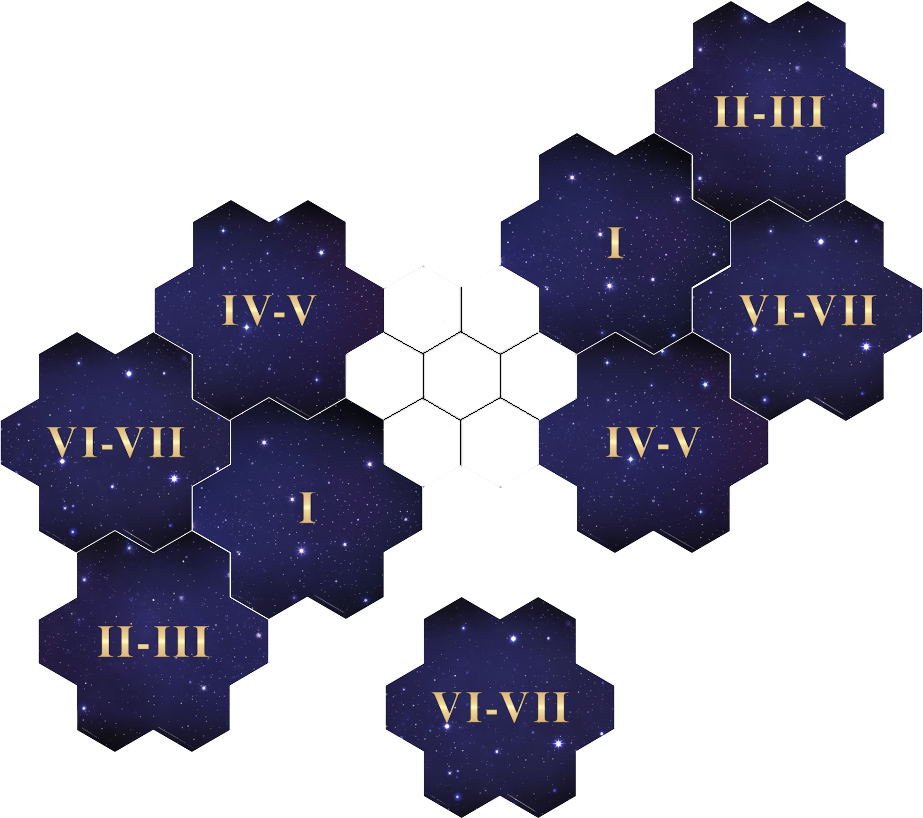
\includegraphics[width=1.0\linewidth]{\maps/king_of_the_hill_v2-2p.png}
  \captionof{figure}{\textbf{2-PLAYER SCENARIO}}
  \vfill
  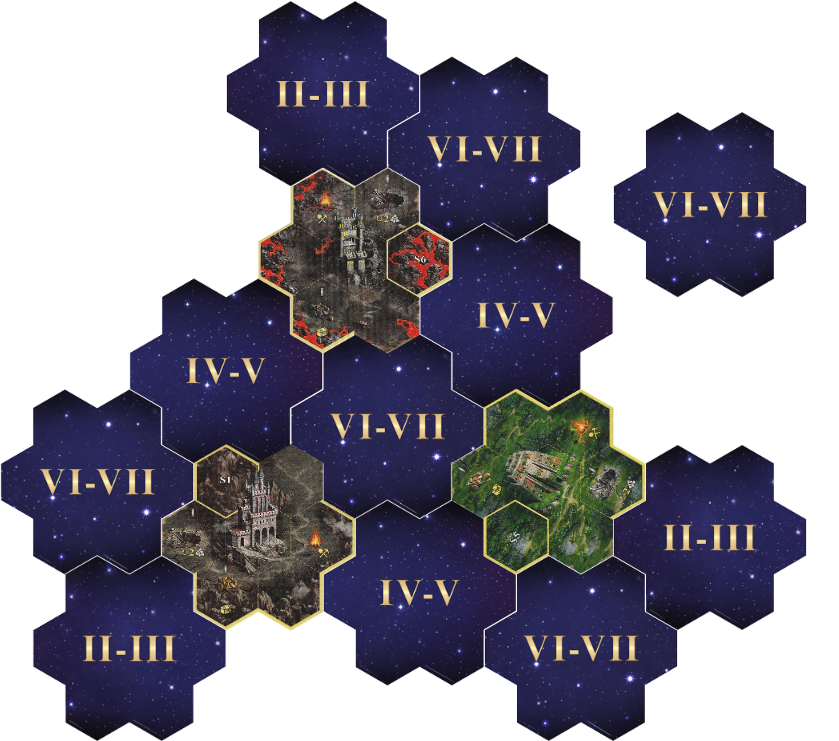
\includegraphics[width=1.0\linewidth]{\maps/king_of_the_hill_v2-3p.png}
  \captionof{figure}{\textbf{3-PLAYER SCENARIO}}
\end{center}

\end{multicols*}
